\documentclass[11pt,a4paper]{article}

\usepackage[margin=2.5cm]{geometry}
\usepackage{booktabs}
\usepackage{graphicx}
\usepackage{hyperref}
\usepackage{xcolor}
\usepackage{tikz}
\usetikzlibrary{arrows.meta,positioning,shapes.geometric}
\usepackage{amsmath}
\usepackage[numbers]{natbib}
\usepackage{enumitem}
\usepackage{tabularx}
\usepackage{float}

\hypersetup{
    colorlinks=true,
    linkcolor=blue!60!black,
    citecolor=blue!60!black,
    urlcolor=blue!60!black
}

\title{A Connection-Based Memory Lifecycle for AI Coding Assistants}
\author{Thomas Pittinger}
\date{March 2026}

\begin{document}

\maketitle

\begin{abstract}
LLM coding assistants accumulate memory entries across sessions but lack mechanisms for forgetting, consolidation, or quality control.
We analyzed 3,874 memory entries from daily use of Claude Code and found three root problems: no schema, no lifecycle process, and no automation.
From this analysis, we designed and implemented a connection-based memory lifecycle system that operates as a meta-layer across five existing memory systems.
The system uses local embeddings (Qwen3-0.6B, ONNX INT8) to track connections between entries; entries that connect to other knowledge survive consolidation, while isolated entries face a substance check and either receive protection or fade.
The entire system runs through Claude Code's hooks API with zero modifications to the tool itself.
We report design decisions with rejected alternatives, and a self-evaluation across 9 automated metrics from 28 sessions of real use.
This is a practitioner's report, not a benchmark paper: the system optimizes for lifecycle quality in daily practice, not retrieval accuracy on synthetic datasets.
The system is open source.\footnote{\url{https://github.com/living0tribunal-dev/claude-memory-lifecycle}}
\end{abstract}


% ============================================================
\section{Introduction}
% ============================================================

Large language model coding assistants generate and consume knowledge across sessions.
Claude Code, Cursor, Windsurf, and GitHub Copilot all maintain some form of persistent memory, from flat markdown files to structured databases.
The common pattern is accumulation: entries are added but rarely removed, consolidated, or validated.

We encountered this problem firsthand.
After several months of daily Claude Code use, the legacy memory system contained 3,874 entries.
80\% lacked any tags.
81\% originated from a single month.
Only 32\% had embeddings, meaning semantic search could not find two-thirds of all entries.
Session logs outnumbered actual knowledge.
The system stored everything and forgot nothing.

This report describes a memory lifecycle system we designed and built over 28 iterative sessions.
The methodology was bottom-up: we started from the data, identified problems, extracted patterns, designed an architecture, implemented it in five phases, and evaluated the result empirically.
We chose the Technical Report format deliberately.
The system has no controlled user study and no benchmark results against LoCoMo~\cite{maharana2024locomo}, LongMemEval, or similar datasets.
Those benchmarks measure retrieval accuracy on synthetic multi-session dialogues; our system optimizes for a different goal, namely memory lifecycle quality in real daily use.
A Technical Report matches this contribution honestly: a practitioner's system with design decisions and lessons learned.


% ============================================================
\section{From Data to Design}
% ============================================================

\subsection{Symptoms}

Analysis of the 3,874 legacy entries revealed 11 symptoms.
Table~\ref{tab:symptoms} shows how they cluster into three root problems.

\begin{table}[h]
\centering
\caption{11 symptoms converging on 3 root problems.}
\label{tab:symptoms}
\small
\begin{tabularx}{\textwidth}{lXl}
\toprule
\textbf{\#} & \textbf{Symptom} & \textbf{Root} \\
\midrule
1 & 80\% of entries untagged; retrieval depends on manual annotation & Schema \\
2 & Temporal explosion (81\% from one month, 575 in a single day) & Lifecycle \\
3 & Embedding gap (32\%); semantic search blind to two-thirds of entries & Automation \\
4 & No process between storing and retrieving & Lifecycle \\
5 & Pseudo-categorization; no data model or enforced schema & Schema \\
6 & System feeds itself noise (auto-save on every context compaction) & Lifecycle \\
7 & No recall tracking; no feedback on whether memory was useful & Automation \\
8 & No write gate; no duplicate or relevance check & Lifecycle \\
9 & Memory and project knowledge stored separately, no integration & Schema \\
10 & $O(n)$ retrieval everywhere; loads all documents into memory & Automation \\
11 & No knowledge classes; everything is a ``document'' & Schema \\
\bottomrule
\end{tabularx}
\end{table}

\textbf{No schema:} entries were flat text blobs with no structured metadata.
Tags existed only as substrings, with no index and no enforcement.
924 unique ``tags'' included noise like \texttt{\#2}, \texttt{\#1}, and \texttt{\#10373}.

\textbf{No lifecycle:} there was no process between storing and retrieving.
Every entry persisted indefinitely regardless of relevance, accuracy, or redundancy.

\textbf{No automation:} everything depended on manual intervention.
Tagging, cleanup, and relevance assessment were all human tasks that did not scale.


\subsection{Pattern: Meta-Layer, Not a Sixth Store}

Claude Code already operates five memory systems (Table~\ref{tab:five-systems}).
The initial instinct was to build a better database.
But the data pointed elsewhere: the problem was not storage capacity or query speed.
The problem was that no process managed the lifecycle across these five systems.
Knowledge was siloed, duplicated, and stale because nothing orchestrated it.

\begin{table}[h]
\centering
\caption{Five existing memory systems in Claude Code.}
\label{tab:five-systems}
\small
\begin{tabular}{lll}
\toprule
\textbf{System} & \textbf{Memory Type} & \textbf{Function} \\
\midrule
Rules files & Procedural & Control behavior via hooks \\
CLAUDE.md & Working memory & Per-project context \\
\_RESEARCH/ & Declarative/Semantic & Research knowledge \\
Git history & Version memory & Change history \\
claude-mem & Episodic & Long-term learnings \\
\bottomrule
\end{tabular}
\end{table}

This reframed the design target: instead of a new store, we needed a \emph{meta-layer}, a knowledge orchestrator that manages lifecycle across all existing systems.
Six initially identified meta-tasks (routing, deduplication, consistency, lifecycle, anticipation, stop-signal) collapsed during design into three operations: \emph{staging} (buffer with lifecycle states), \emph{consolidation} (LLM-powered merging with routing), and \emph{anticipation} (proactive briefing with consistency checking).


\subsection{Broken Assumptions}

A structured perspective-taking exercise (12 domain perspectives plus a deliberate assumption-breaking pass) revealed 8 implicit assumptions in our original framing.
The three most consequential corrections were:

\begin{enumerate}[nosep]
    \item \textbf{Memory is not a data problem; it is a timing and context problem.} The question is not ``how do we store more'' but ``when does the agent need which knowledge.''
    \item \textbf{More memory is not better.} Beyond a threshold, additional entries compete for context window space and degrade reasoning quality.
    \item \textbf{Everything should be stored} $\rightarrow$ \textbf{Only proven knowledge deserves long-term storage.} Most entries are transient; promoting them prematurely pollutes the knowledge base.
\end{enumerate}


% ============================================================
\section{Architecture}
% ============================================================

\subsection{Five-Phase Lifecycle}

Figure~\ref{fig:pipeline} shows the lifecycle pipeline.
Every entry passes through five phases, though not every entry reaches all of them.

\begin{figure}[h]
\centering
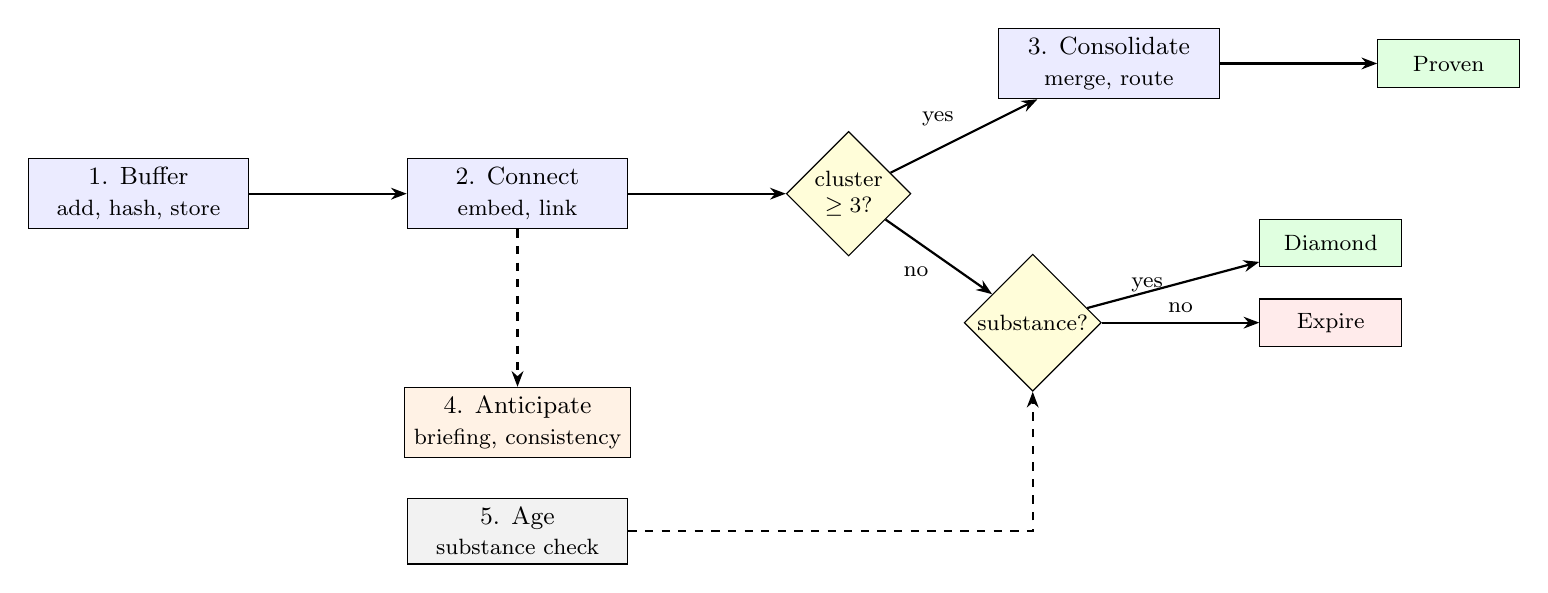
\begin{tikzpicture}[
    node distance=1.2cm and 2cm,
    phase/.style={rectangle, draw, fill=blue!8, minimum width=2.8cm, minimum height=0.8cm, align=center, font=\small},
    decision/.style={diamond, draw, fill=yellow!15, minimum width=1.5cm, minimum height=0.8cm, align=center, font=\footnotesize, inner sep=1pt},
    outcome/.style={rectangle, draw, fill=red!8, minimum width=1.8cm, minimum height=0.6cm, align=center, font=\footnotesize},
    promote/.style={rectangle, draw, fill=green!12, minimum width=1.8cm, minimum height=0.6cm, align=center, font=\footnotesize},
    arr/.style={-{Stealth[length=2mm]}, thick}
]

\node[phase] (buffer) {1. Buffer\\{\footnotesize add, hash, store}};
\node[phase, right=of buffer] (connect) {2. Connect\\{\footnotesize embed, link}};
\node[decision, right=of connect] (cluster) {cluster\\$\geq 3$?};
\node[phase, above right=0.8cm and 1.5cm of cluster] (consolidate) {3. Consolidate\\{\footnotesize merge, route}};
\node[decision, below right=0.8cm and 1.5cm of cluster] (isolated) {substance?};
\node[promote, right=of consolidate] (proven) {Proven};
\node[outcome, right=of isolated] (expire) {Expire};
\node[promote, above=0.4cm of expire] (diamond) {Diamond};

\draw[arr] (buffer) -- (connect);
\draw[arr] (connect) -- (cluster);
\draw[arr] (cluster) -- node[above left, font=\footnotesize]{yes} (consolidate);
\draw[arr] (cluster) -- node[below left, font=\footnotesize]{no} (isolated);
\draw[arr] (consolidate) -- (proven);
\draw[arr] (isolated) -- node[above, font=\footnotesize]{no} (expire);
\draw[arr] (isolated) -- node[left, font=\footnotesize]{yes} (diamond);

\node[phase, below=2cm of connect, fill=orange!10] (anticipate) {4. Anticipate\\{\footnotesize briefing, consistency}};
\node[phase, below=0.5cm of anticipate, fill=gray!10] (age) {5. Age\\{\footnotesize substance check}};

\draw[arr, dashed] (connect.south) -- (anticipate.north);
\draw[arr, dashed] (age.east) -| (isolated.south);

\end{tikzpicture}
\caption{Memory lifecycle pipeline. Solid arrows show the primary flow; dashed arrows show secondary triggers. Phase 4 (Anticipate) runs on session start or topic switch. Phase 5 (Age) feeds isolated entries into the substance check.}
\label{fig:pipeline}
\end{figure}

\textbf{Phase 1, Buffer:} every entry enters without judgment.
A SHA256 hash prevents exact duplicates.
No model runs at write time; latency stays under 50\,ms.

\textbf{Phase 2, Connect:} a batch process embeds all pending entries using Qwen3-0.6B (ONNX INT8, local, no API call) and computes pairwise cosine similarities.
Entries with similarity above 0.75 are linked in a connection graph stored in SQLite.

\textbf{Phase 3, Consolidate:} connected components with 3 or more entries form clusters.
A token-overlap heuristic (Jaccard on word sets) distinguishes noise clusters (session logs with over 80\% word overlap) from knowledge clusters.
Knowledge clusters are merged by an LLM into a single proven entry that also receives a routing target and a conflict check against existing content.
Original entries expire after successful consolidation.

\textbf{Phase 4, Anticipate:} on session start or topic switch, the system embeds the current context (from the project's RESUME\_PROMPT.md) and retrieves the most similar buffer entries.
A secondary consistency check flags contradictions among loaded entries.
No additional API call is needed; the system reuses existing embeddings.

\textbf{Phase 5, Age:} entries that remain isolated after all embeddings are computed face a substance check.
An LLM evaluates whether the entry contains genuine standalone knowledge.
Valuable isolates receive a reprieve (up to 3 times).
User thoughts and decisions are protected and never auto-expire.


\subsection{Design Decisions}

Each decision emerged from data analysis or structured red-teaming, not from a prior framework.
Table~\ref{tab:decisions} summarizes all seven with their rationale and rejected alternatives.

\begin{table}[H]
\centering
\caption{Seven design decisions with rationale and rejected alternatives.}
\label{tab:decisions}
\small
\begin{tabularx}{\textwidth}{lXX}
\toprule
\textbf{Decision} & \textbf{Rationale} & \textbf{Rejected Alternative} \\
\midrule
Staging over Gate & Value is unknown at write time; it reveals itself through connections & LLM write-time gate (failed in red-teaming: best insights lack signal words) \\
\addlinespace
Connection-based expiry & Isolation determines decay, not time; long-lived knowledge survives & TTL / Ebbinghaus curves (destroy old-but-referenced knowledge) \\
\addlinespace
Two promotion modes & Cluster-only penalizes uniqueness; diamond protection rescues isolates & Single-path promotion (red-team attack showed unique insights would expire) \\
\addlinespace
Mechanical noise detection & Token overlap $>$80\% identifies template clusters without LLM & LLM-based noise classification (unnecessary cost for a deterministic signal) \\
\addlinespace
Unified consolidation & One LLM call for merging, routing, dedup, and conflict check & Separate calls per task (higher cost, same input context) \\
\addlinespace
Embedded anticipation & Enriched embedding context (RESUME\_PROMPT) eliminated need for LLM ranking & Separate LLM ranking step (empirical test: context enrichment raised similarity from 0.40 to 0.74) \\
\addlinespace
Lazy migration & Useful legacy entries migrate through recall; noise stays in archive & Batch import of 3,874 entries (expensive, unclear benefit) \\
\bottomrule
\end{tabularx}
\end{table}


\subsection{Two-Speed Architecture}

The system separates high-frequency deterministic operations from low-frequency LLM-powered operations:

\begin{itemize}[nosep]
    \item \textbf{Every entry:} embedding (ONNX, local), cosine similarity, token overlap, connection tracking. Deterministic, no API dependency.
    \item \textbf{At promotion time only:} consolidation, routing, conflict check, substance check. LLM-powered, typically a few times per day.
\end{itemize}

This separation ensures that the system functions without an API connection for its core operations.
LLM calls are reserved for the infrequent, high-value decisions where human-level judgment matters.


\subsection{Quality Assurance Layer}

A separate LLM reviews the coding assistant's output after every response, checking against methodology rules.
This is a mechanism, not a prompt: the assistant cannot ignore it because it runs outside the assistant's context window.

The checker uses two hook events.
On \texttt{Stop} (after the assistant responds), it evaluates the response against 5 rules and writes violations to a temporary file.
On the next \texttt{UserPromptSubmit} (before the assistant sees the user's message), it reads the file and injects violations as system context.

The assistant receives violation feedback in the same channel as system instructions.
The rules are enforced at the mechanism level (external hook plus separate LLM), not the prompt level (instruction within the assistant's context).
The default checker model is Gemini 3.1 Flash-Lite on the free tier, providing approximately 1,000 checks per day.


\subsection{Hook-Based Integration}

The entire system runs through Claude Code's hooks API~\cite{claudecodehooks}, requiring zero modifications to the tool.
Table~\ref{tab:hooks} shows the mapping.

\begin{table}[h]
\centering
\caption{Hook events and their functions.}
\label{tab:hooks}
\small
\begin{tabularx}{\textwidth}{lX}
\toprule
\textbf{Hook Event} & \textbf{What Runs} \\
\midrule
UserPromptSubmit & Context injection, focus checks, violation feedback, write-gate reset \\
PreToolUse & 3-gate safety checks, write-gate enforcement \\
PostToolUse & Read tracking, agent result persistence \\
Stop & Self-checks, Gemini quality checker (async) \\
PreCompact & Session save, embedding updates, aging pipeline, graceful shutdown \\
\bottomrule
\end{tabularx}
\end{table}

This constraint was deliberate.
Any system that requires forking or modifying the host tool becomes unmaintainable across updates.
Hooks are the official extension point; they survive version upgrades without changes to the lifecycle system.


% ============================================================
\section{Key Engineering Decisions}
% ============================================================

\subsection{Embedding Model Selection}

We evaluated four embedding models against our hardware constraint (6\,GB RAM laptop, Intel i5-8250U, no GPU).
Table~\ref{tab:embeddings} summarizes the comparison.

\begin{table}[h]
\centering
\caption{Embedding model comparison. MMTEB scores are multilingual.}
\label{tab:embeddings}
\small
\begin{tabular}{lcccc}
\toprule
\textbf{Model} & \textbf{MMTEB} & \textbf{Dim} & \textbf{RAM} & \textbf{License} \\
\midrule
all-MiniLM-L6-v2 & $\sim$56 & 384 & $\sim$100\,MB & Apache 2.0 \\
BGE-M3 & 59.56 & 1024 & $\sim$2.2\,GB & MIT \\
EmbeddingGemma-300M & 61.15 & 768 & $\sim$1.2\,GB & Gemma \\
\textbf{Qwen3-0.6B (INT8)} & \textbf{64.33} & \textbf{1024} & \textbf{$\sim$560\,MB} & \textbf{Apache 2.0} \\
\bottomrule
\end{tabular}
\end{table}

Qwen3-Embedding-0.6B~\cite{qwen3embedding} scored highest on MMTEB Multilingual and offered ONNX INT8 quantization fitting our RAM constraint.
A structured red-teaming process revealed two critical issues with EmbeddingGemma-300M: silent incorrect similarity scores with the wrong \texttt{transformers} version (confirmed via HuggingFace discussion), and a 164x slowdown on text containing whitespace (confirmed via upstream issue tracker).

We use the full 1024-dimensional embeddings despite the model's Matryoshka support for reduced dimensions.
Empirical testing by Sack~\cite{matryoshkawarning} showed that 256-dimensional Matryoshka embeddings retain only 57\% of top-10 retrieval overlap compared to the full dimension.
For connection tracking, where borderline similarities determine cluster membership versus isolation, this loss is unacceptable.


\subsection{Diamond Protection}

Standard lifecycle systems offer two outcomes for an entry: consolidation (if it clusters) or expiry (if it does not).
This penalizes genuinely unique knowledge.
Diamond protection adds a third outcome: reprieve.

Before expiring an isolated entry, the system runs a substance check.
The question is simple: does this entry contain specific, actionable knowledge?
Entries that pass receive a reprieve (up to 3 times).
Entries that fail expire.
User thoughts and decisions are exempt from expiry entirely, as a hard rule rather than a probabilistic judgment.

Unlike permanent-memory flags where the user must predict importance upfront, diamond protection discovers valuable isolates automatically during the aging process.


\subsection{Memory Type Classification}

Entries are classified into five types at write time using deterministic pattern matching, requiring no LLM (Table~\ref{tab:types}).

\begin{table}[h]
\centering
\caption{Memory types with detection patterns and lifecycle behavior.}
\label{tab:types}
\small
\begin{tabularx}{\textwidth}{llX}
\toprule
\textbf{Type} & \textbf{Detection} & \textbf{Lifecycle Behavior} \\
\midrule
decision & \texttt{\#decision} tag & Never auto-expires (format: what + because + consequence) \\
user-gedanke & \texttt{\#user-gedanke} tag & Never auto-expires (user's explicit thoughts) \\
session-save & \texttt{\#session-save} tag & Normal lifecycle: consolidation and aging \\
auto-session-save & \texttt{AUTO-SESSION-SAVE} prefix & Immediately expired if empty (0 user messages) \\
insight & None of the above & Normal lifecycle \\
\bottomrule
\end{tabularx}
\end{table}

The classification drives lifecycle behavior mechanically.
Empty auto-session-saves expire at write time.
User thoughts and decisions receive permanent protection.
Session saves follow normal consolidation and aging.
This removes entire categories of noise without manual intervention.


% ============================================================
\section{Self-Evaluation}
% ============================================================

We validate the system using 9 automated checks against the live database.
These metrics test whether the lifecycle mechanisms function correctly, not retrieval accuracy.
Table~\ref{tab:eval} shows the results.

\begin{table}[h]
\centering
\caption{Evaluation results from the live database after 28 sessions.}
\label{tab:eval}
\small
\begin{tabularx}{\textwidth}{llX}
\toprule
\textbf{Metric} & \textbf{Result} & \textbf{What It Checks} \\
\midrule
Cross-project connections & 0 & Write-time filter prevents false links between unrelated projects \\
Type detection accuracy & 71/71 (100\%) & Deterministic classifier matches expected type for every entry \\
Auto-expire precision & 0\,FP, 0\,FN & Empty auto-session-saves expire; non-empty ones survive \\
User-gedanke protection & 5/5 protected & User's explicit thoughts never auto-expire \\
Connection discrimination & 276 intra, 0 cross & Connections form within projects, not across them \\
Cluster density & 93\% connected & Most buffer entries link to at least one other entry \\
Promotion rate & 5.6\% & Selective: only well-connected knowledge advances to proven \\
Aging audit & 24 expired & Expired entries are empty saves (8), old session-saves (10), unlinked (6) \\
Recall tracking & 5 recalled & Search-driven recall counts feed the promotion pathway \\
\bottomrule
\end{tabularx}
\end{table}


\subsection{Limitations}

\textbf{No formal benchmarks.}
We did not evaluate against LoCoMo~\cite{maharana2024locomo}, LongMemEval, or MemoryBench.
Those benchmarks measure retrieval accuracy on synthetic multi-session dialogues.
Our system optimizes for lifecycle quality (correct expiry, correct routing, correct consolidation) in real daily use.
This limits comparability with systems that report benchmark numbers.

\textbf{Single user.}
The system was designed for and tested by one person across 28 sessions.
We cannot claim generalizability to other users, workflows, or tools.

\textbf{LLM dependency.}
Consolidation and quality checking require an LLM API.
The default Gemini free tier works within rate limits for moderate use (15 to 25 sessions per day).
Heavier use would require a paid API or a local LLM.

\textbf{Claude Code specific.}
The hooks API is specific to Claude Code.
Adapting the system to other tools requires reimplementing the integration layer, though the core lifecycle logic is tool-agnostic.


% ============================================================
\section{Related Work}
% ============================================================

\subsection{Systems Comparison}

We surveyed 17 memory systems for LLM coding assistants~\cite{liu2024memory, mem0paper, simplemem, memospaper}.
Table~\ref{tab:comparison} positions our system among the most relevant.

\begin{table}[H]
\centering
\caption{Comparison with selected memory systems.}
\label{tab:comparison}
\small
\begin{tabularx}{\textwidth}{lXlll}
\toprule
\textbf{System} & \textbf{Memory Model} & \textbf{Expiry} & \textbf{Quality Check} & \textbf{Integration} \\
\midrule
This system & Connection-based lifecycle & Isolation + substance & LLM cross-check & Hooks \\
engram-rs~\cite{engramrs} & Buffer/Working/Core & Epoch decay & LLM quality gate & MCP + CLI \\
engram-ai~\cite{engramai} & 5-type knowledge graph & Ebbinghaus + exemptions & Noise gate & MCP \\
SimpleMem~\cite{simplemem} & CLS-theory & Decay function & Benchmarked & Research \\
MemOS~\cite{memospaper} & Governance + TTL & Time + policy & Conflict detection & Framework \\
Copilot Memory & Citation-verification & 28d TTL & Self-healing & Built-in \\
Claude auto-memory & Flat files, append-only & None & None & Built-in \\
\bottomrule
\end{tabularx}
\end{table}

Across the 17 surveyed systems, the most common feature is consolidation (13 of 17).
Forgetting or decay mechanisms appear in 8 of 17.
Runtime validation is rare (3 of 17), and cross-system conflict detection appears in only 2 of 17.

Our closest competitor in architecture is engram-rs, which implements a three-layer system (Buffer, Working Memory, Core) with an LLM quality gate and epoch-based decay, covering 5.5 of our 6 lifecycle stages.
The primary differences are our connection-based (rather than time-based) expiry, our project isolation mechanism, and our external quality checker running a separate LLM.

We do not claim that our system is more comprehensive than all alternatives.
MemOS, for example, has fewer phases but offers governance policies, compliance features, and TTL-based management that our system lacks.
Our contribution is specific: a practitioner's implementation of connection-based lifecycle management with diamond protection, built entirely on hooks.


\subsection{Theoretical Connection}

The system's architecture maps to Complementary Learning Systems (CLS) theory~\cite{mcclelland1995cls}: the buffer corresponds to fast hippocampal learning, persistent storage corresponds to slow neocortical integration, and the consolidation pipeline corresponds to hippocampal replay.
Connected memories survive replay; isolated ones do not.

We state this connection honestly: it was recognized after the fact, not used as a design principle.
We designed bottom-up from data, and the resulting architecture happened to mirror CLS.
Any system with a buffer-to-persistent-storage pattern could claim a similar connection.
SimpleMem~\cite{simplemem} and HiCL~\cite{hicl} implement CLS explicitly, with formal mappings and benchmark evaluations that our system does not provide.

The more interesting observation is convergence: starting from practical problems (noise, no lifecycle, no forgetting) and working bottom-up led to an architecture that independently resembles what neuroscience suggests about biological memory consolidation.
Whether this reflects a deep structural constraint or simply the obviousness of buffer-plus-consolidation as a pattern is an open question.


% ============================================================
\section{Conclusion}
% ============================================================

We presented a connection-based memory lifecycle system for Claude Code that addresses three root problems in LLM memory: no schema, no lifecycle, and no automation.
The system operates as a meta-layer across five existing memory systems, using local embeddings for connection tracking and an external LLM for consolidation and quality checking.

The central design insight is that memory expiry should be driven by isolation, not time.
Entries that connect to other knowledge survive.
Entries that remain isolated face a substance check and either receive protection or fade.
This approach emerged bottom-up from analyzing real data rather than from applying a theoretical framework.

The system has been in daily use for 28 sessions.
It runs entirely through Claude Code's hooks API, requires no modification to the host tool, and is open source.
The core lifecycle logic (buffer, connect, consolidate, route, age) is tool-agnostic; only the hook integration layer is Claude Code specific.


% ============================================================
% Technology summary
% ============================================================

\subsection*{Technology Stack}

\begin{table}[h]
\centering
\small
\begin{tabular}{ll}
\toprule
\textbf{Component} & \textbf{Choice} \\
\midrule
Buffer store & SQLite (WAL mode) \\
Embeddings & Qwen3-0.6B ONNX INT8, 1024 dimensions \\
Consolidation LLM & Any with JSON mode (default: Gemini Flash, free tier) \\
Quality checker LLM & Any with chat API (default: Gemini 3.1 Flash-Lite, free tier) \\
Integration & Claude Code hooks API (zero modification) \\
Codebase & Single Python script ($\sim$2,300 lines) plus hook scripts \\
Dependencies & SQLite, ONNX Runtime, transformers tokenizer \\
\bottomrule
\end{tabular}
\end{table}


% ============================================================
% References
% ============================================================

\begin{thebibliography}{20}

\bibitem{mcclelland1995cls}
J.~L. McClelland, B.~L. McNaughton, and R.~C. O'Reilly,
``Why there are complementary learning systems in the hippocampus and neocortex: Insights from the successes and failures of connectionist models of learning and memory,''
\emph{Psychological Review}, vol.~102, no.~3, pp.~419--457, 1995.

\bibitem{liu2024memory}
Z.~Liu et al.,
``Memory in the age of LLM-based agents,''
\emph{arXiv preprint arXiv:2512.13564}, 2024.

\bibitem{mem0paper}
Mem0 Authors,
``Mem0: Building production-ready AI agents with scalable long-term memory,''
\emph{arXiv preprint arXiv:2504.19413}, 2025.

\bibitem{simplemem}
SimpleMem Authors,
``SimpleMem: Towards semantic lossless LLM memory compression,''
\emph{arXiv preprint arXiv:2601.02553}, 2026.

\bibitem{memospaper}
MemOS Authors,
``MemOS: An operating system for LLM agents with governance,''
\emph{arXiv preprint arXiv:2505.22101}, 2025.

\bibitem{memorybank}
Z.~Zhong et al.,
``MemoryBank: Enhancing large language models with long-term memory,''
\emph{AAAI}, 2024.
\emph{arXiv preprint arXiv:2305.10250}.

\bibitem{amem}
W.~Xu et al.,
``A-MEM: Agentic memory for LLM agents,''
\emph{NeurIPS}, 2025.
\emph{arXiv preprint arXiv:2502.12110}.

\bibitem{hicl}
HiCL Authors,
``HiCL: Hippocampus-inspired complementary learning for agentic memory,''
\emph{AAAI}, 2025.
\emph{arXiv preprint arXiv:2508.16651}.

\bibitem{maharana2024locomo}
A.~Maharana et al.,
``Evaluating very long-term conversational memory of LLM agents,''
\emph{ACL}, 2024.

\bibitem{engramrs}
kael-bit,
``engram-rs: Rust-based memory system with Atkinson-Shiffrin three-layer architecture,''
\url{https://github.com/kael-bit/engram-rs}, 2025.

\bibitem{engramai}
foramoment,
``engram-ai-memory: SQLite-based memory with Ebbinghaus decay,''
\url{https://github.com/foramoment/engram-ai-memory}, 2025.

\bibitem{qwen3embedding}
Qwen Team,
``Qwen3-Embedding-0.6B,''
\url{https://huggingface.co/Qwen/Qwen3-Embedding-0.6B}, 2025.

\bibitem{matryoshkawarning}
J.~Sack,
``Matryoshka embeddings: Benchmark quality vs. practical retrieval overlap,''
\url{https://joesack.substack.com/p/matryoshka-embeddings-benchmark-quality}, 2025.

\bibitem{claudecodehooks}
Anthropic,
``Claude Code hooks,''
\url{https://docs.anthropic.com/en/docs/claude-code/hooks}, 2025.

\bibitem{knowledgeconflicts}
R.~Xu et al.,
``Knowledge conflicts for LLMs: A survey,''
\emph{EMNLP}, 2024.

\bibitem{copilotmemory}
GitHub,
``Building an agentic memory system for GitHub Copilot,''
\url{https://github.blog/ai-and-ml/github-copilot/building-an-agentic-memory-system-for-github-copilot/}, 2025.

\end{thebibliography}

\end{document}
